\chapter{Background}
\label{chap:background}

This chapter describes the theoretical concepts of importance for the thesis: it explains information and communication and the difference between the two, presents the notions of heat maps and social networks, and gives a brief introduction to agile software development's core values.

\section{Communication \& Information}
\label{chap:background-comm-info}

Communication is the exchange of meaning between various parties. Within this exchange, the medium's specific channel type or physical nature to exchange meaning is not of interest in most theories~\citep{savage2011informationtheory}.~\citet{shannon1948theoryofcommunication}, as illustrated in Figure \ref{fig:communication-system}, defines a model which envisions the role of a transmitter and receiver between which the signal is transferred while being prone to potential external noise. Internal noise, on the other hand, can emerge during the encoding or decoding process of a sender or receiver~\citep{verdu1998informationtheory}.
In addition, messages are exposed to an exponentially increasing amount of noise in relation to the nodes they pass through. This specially applies for large organisations with long distances between the sender and final receiver~\citep{shannon1948theoryofcommunication}.

\begin{figure}[h!]
  \centering
  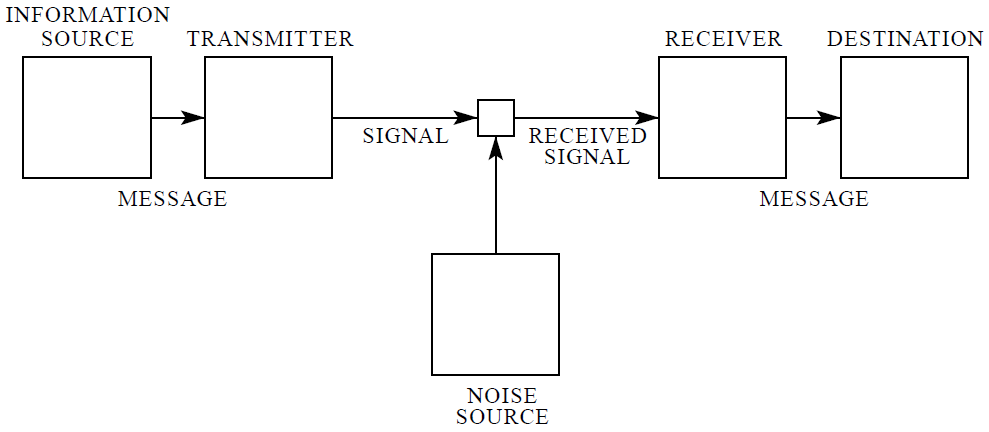
\includegraphics[width=0.90\textwidth]{figures/communication-information-shannon.png}
  \caption{Schematic diagram of a general communication system~\citep{shannon1948theoryofcommunication}}
  \label{fig:communication-system}
\end{figure}

Information coheres to communication as it is perceived as the message which travels between parties~\citep{floridiinformationintro}. Just as~\citet{savage2011informationtheory} attempts to embed communication in a mathematical model, information theory formalises areas of signal processing and data compression. Signals are not independent of their context and static in how they are understood during interpretation before their transmission~\citep{vigo2011representionalinformation}. Whenever a single piece of information is accessed, a human processes it, which is a dynamic procedure strongly influenced by the context of the actor and its ability to understand the information's complexity~\citep{vigo2011representionalinformation}. Finally, whenever the meaning conveyed constitutes something previously unknown,~\citet{gleick2012theinformation} acknowledges actual information being transmitted.

In the scope of this thesis the concepts linked to information and communication are being handled separately. \textit{Communication} is understood as a form of humans dynamically exchanging information through various channels where \textit{information} is a single manifestation of a message's content.

\section{Heat Maps}

Heat maps were first used over a century ago to illustrate social statistics across various districts in France~\citep{friendly09thehistory}. 
Over time statisticians have worked on different algorithms to perform various types of clusterings involving permutations of the heat maps' rows and columns~\citep{friendly09thehistory}, allowing the heat map to be more powerful visualisation tool communicating the data's statement clearly.
As a result, heat maps are often used to visualise dense, three-dimensional data of a table format. Data in regards to an observation can be collected continuously over or at a discrete point in time~\citep{gehlensborg2012heatmaps}.
Colour coding is then used to give structure and illustrate clusterings. All in all, it allows for an easier interpretation of the original data~\citep{gehlensborg2012heatmaps}. Their data independence allows heat maps to be applied in different fields such as social science, biology or meteorology.

In software engineering~\citet{feldt2013heatmaps} use heat maps to visualise code churns over time of different code elements to predict potential integration problems. Other investigations visualise the change status with a file and project view using colour coding for each line's status~\citep{voinea2007visualassessment}. The aggregated project view gives a dense view of the overall status also linking progress to single developers.
\citet{coplien1996patternsofprod} utilise heat maps to visualise the intensity of communication between roles within software development organisations. Their heat maps, which are called interaction grids, are sorted in descending order according to the roles' communication intensities, illustrating the epicentre of communication and the associated roles at the point of origin. By performing further analysis and data comparisons,~\citet{coplien1996patternsofprod} deduct characteristics of successful corporations such as inward communication flow, even distribution of work and the distribution of communication among roles.

Heat maps are used in the context of this thesis to demonstrate the intensities of communications of different natures between the representatives of various roles in an organisation.

\section{Social Networks}

Social networks are a concept vastly used in sociology as a mean to represent social groups as networks of their interrelations. Their analysis has been mathematically formalised and, as outlined by \citet{scott2011sn}, is closely related to the methods of graph theory. Using the terminology of the latter, individuals (or groups of individuals) in a social network are represented as nodes while their interrelations are depicted by edges. \citet{scott2011sn} mentions the measures of network density and centrality, examination of cliques and clusters as a few aspects of a social network that can be investigated using existing methods and theories.

Linguistics, criminology and demography are among other research areas that over time incorporated the analysis of social networks in their field of study. 

In software engineering's body of knowledge, social networks have been used for instance by \citet{Cataldo2008} for communication analysis in a geographically~\ac{DSD} to study the core of communication networks and the level of technical proficiency of those in the core. 

The thesis employs social networks to complement the heat maps visualisations with a structured overview of the communication paths between the representatives of various roles in an organisation.

\section{Agile's Principles \& Values}

Almost all agile practices and methodologies are based on a set of common values and principles. The original proclamation of agile's values in \quotes{The Agile Manifesto} states four core values~\citep{beck2001agile}:

\begin{description}
  \item[Individuals and interactions] over processes and tools.
  \item[Working software] over comprehensive documentation.
  \item[Customer collaboration] over contract negotiation.
  \item[Responding to change] over following a plan.
\end{description}

The values are contemplated with 12 principles which themselves are build around three main categories: delivery, communication and quality~\citep{beck2001agile}. By taking both, values and principles, into account the community around them termed various agile methods, such as Scrum~\citep{sims2012scrum},~\ac{XP}~\citep{beck2004xp} and the Crystal methodologies~\citep{cockburn2004crystal}. These extend agile's basic notion by custom foundations such as Scrum's five values in commitment, focus, openness, respect, courage~\cite{schwaberagilescrum}.

The studied organisation employs agile methodologies based upon the stated values by which they impact the work environment and participants under study. 